\chapter{Практический раздел}

\section{Листинг алгоритма MD5}

\begin{lstlisting}[language=C, label=lst:md5, caption={Реализация алгоритма MD5}]
typedef struct {
    uint64_t cur_len;
    uint8_t cur_input[64];

    uint32_t parts[4];

    uint8_t digest[16];
} hasher_t;

void init(hasher_t *h) {
    h->cur_len = (uint64_t) 0;

    h->parts[0] = 0x67452301;
    h->parts[1] = 0xefcdab89;
    h->parts[2] = 0x98badcfe;
    h->parts[3] = 0x10325476;
}

void step(uint32_t *buf, const uint32_t *input) {
    uint32_t a = buf[0];
    uint32_t b = buf[1];
    uint32_t c = buf[2];
    uint32_t d = buf[3];

    for (unsigned int i = 0; i < 64; i++) {
        uint32_t f, g;

        if (i <= 15) {
            f = (b & c) | (~b & d);
            g = i % 16;
        }
        else if (i <= 31) {
            f = (b & d) | (c & ~d);
            g = ((i * 5) + 1) % 16;
        }
        else if (i <= 47) {
            f = (b ^ c ^ d);
            g = ((i * 3) + 5) % 16;
        }
        else {
            f = (c ^ (b | ~d));
            g = (i * 7) % 16;
        }

        f = f + a + k[i] + input[g];
        a = d;
        d = c;
        c = b;
        b = b + rotate_left(f, s[i]);
    }

    buf[0] += a;
    buf[1] += b;
    buf[2] += c;
    buf[3] += d;
}

void update(hasher_t *h, const uint8_t *buf, size_t len) {
    uint32_t input[16];
    uint64_t offset = h->cur_len % 64;
    h->cur_len += (uint64_t) len;

    for (unsigned int i = 0; i < len; i++) {
        h->cur_input[offset++] = buf[i];

        if (offset % 64 == 0) {
            for (unsigned int j = 0; j < 16; ++j) {
                input[j] = (uint32_t) (h->cur_input[(j * 4) + 3]) << 24 |
                           (uint32_t) (h->cur_input[(j * 4) + 2]) << 16 |
                           (uint32_t) (h->cur_input[(j * 4) + 1]) << 8 |
                           (uint32_t) (h->cur_input[(j * 4)]);
            }
            step(h->parts, input);
            offset = 0;
        }
    }
}

void finalize(hasher_t *h) {
    uint32_t input[16];
    unsigned int offset = h->cur_len % 64;
    unsigned int padding_length = offset < 56 ? 56 - offset : (56 + 64) - offset;

    update(h, padding, padding_length);
    h->cur_len -= (uint64_t) padding_length;

    for (unsigned int j = 0; j < 14; ++j) {
        input[j] = (uint32_t) (h->cur_input[(j * 4) + 3]) << 24 |
                   (uint32_t) (h->cur_input[(j * 4) + 2]) << 16 |
                   (uint32_t) (h->cur_input[(j * 4) + 1]) << 8 |
                   (uint32_t) (h->cur_input[(j * 4)]);
    }
    input[14] = (uint32_t) (h->cur_len * 8);
    input[15] = (uint32_t) ((h->cur_len * 8) >> 32);

    step(h->parts, input);

    for (unsigned int i = 0; i < 4; ++i) {
        h->digest[(i * 4) + 0] = (uint8_t) ((h->parts[i] & 0x000000FF));
        h->digest[(i * 4) + 1] = (uint8_t) ((h->parts[i] & 0x0000FF00) >> 8);
        h->digest[(i * 4) + 2] = (uint8_t) ((h->parts[i] & 0x00FF0000) >> 16);
        h->digest[(i * 4) + 3] = (uint8_t) ((h->parts[i] & 0xFF000000) >> 24);
    }
}
\end{lstlisting}


\section{Листинг алгоритма RSA}

\begin{lstlisting}[language=C, label=lst:rsa, caption={Реализация алгоритма RSA}]
int rsa_with_key(const char *buf, int bytes, rsa_key_t *key, char *result) {
    bignum *res, *plain;
    int enc_bytes;

    plain = from_bin(buf, bytes);
    res = bignum_alloc();
    bignum_pow_mod(res, plain, key->exponent, key->modulus);

    enc_bytes = res->length * sizeof(uint32_t);

    for (int i = 0; i < enc_bytes; i++)
        result[i] = ((char *) res->data)[i];

    bignum_free(res);
    bignum_free(plain);

    return enc_bytes;
}
\end{lstlisting}

\begin{lstlisting}[language=C, label=lst:rsa_keygen, caption={Реализация алгоритма RSA (генерация ключей}]
int rsa_generate_keys(char *private_filename, char *public_filename, int bytes) {
    bignum *p = bignum_alloc();
    bignum *q = bignum_alloc();
    bignum *n = bignum_alloc();
    bignum *d = bignum_alloc();
    bignum *e = bignum_alloc();
    bignum *phi = bignum_alloc();

    random_prime(bytes, p);
    random_prime(bytes, q);

    bignum_multiply(n, p, q);
    bignum_isubtract(p, &NUMS[1]);
    bignum_isubtract(q, &NUMS[1]);
    bignum_multiply(phi, p, q);

    find_e(phi, e);
    find_d(e, phi, d);

    rsa_key_t private = {
        .exponent = e,
        .modulus = n,
    };

    rsa_key_t public = {
        .exponent = d,
        .modulus = n,
    };

    if (rsa_write_key(private_filename, &private) != EXIT_SUCCESS) {
        return EXIT_FAILURE;
    }

    if (rsa_write_key(public_filename, &public) != EXIT_SUCCESS) {
        return EXIT_FAILURE;
    }

    bignum_free(p);
    bignum_free(q);
    bignum_free(phi);

    return EXIT_SUCCESS;
}
\end{lstlisting}


\section{Листинг алгоритма цифровой подписи}

\begin{lstlisting}[language=C, label=lst:rsa, caption={Реализация алгоритма цифровой подписи на основе MD5 и RSA}]
int sign(char *filename, char *sign_filename, char *key_filename) {
    uint8_t hash[1024] = { 0 };
    if (md5(filename, hash) != EXIT_SUCCESS) {
        printf("Cannot compute MD5.\n");
        return EXIT_FAILURE;
    }

    printf("File checksum is ");
    md5_print(hash);
    printf(".\n");

    uint8_t sign_content[1024] = { 0 };
    int size;
    if ((size = rsa(hash, 16, "key", sign_content)) < 0) {
        printf("Cannot compute RSA.\n");
        return EXIT_FAILURE;
    }

    if (write_file(sign_filename, sign_content, size) != EXIT_SUCCESS) {
        printf("Cannot write file.\n");
        return EXIT_FAILURE;
    }

    printf("Sign file is %s.\n", sign_filename);

    return EXIT_SUCCESS;
}

int check(char *filename, char *sign_filename, char *key_filename) {
    uint8_t hash[16] = { 0 };
    if (md5(filename, hash) != EXIT_SUCCESS) {
        printf("Cannot compute MD5.\n");
        return EXIT_FAILURE;
    }
    printf("File checksum is ");
    md5_print(hash);
    printf(".\n");

    uint8_t* sign_content;
    int sign_size;
    if (read_file(sign_filename, &sign_content, &sign_size) != EXIT_SUCCESS) {
        printf("Read sign file.\n");
        return EXIT_FAILURE;
    }

    uint8_t hash_from_sign[1024] = { 0 };
    if (rsa(sign_content, sign_size, key_filename, hash_from_sign) < 0) {
        printf("Cannot compute RSA.\n");
        return EXIT_FAILURE;
    }

    printf("Checksum from sign ");
    md5_print(hash_from_sign);
    printf(".\n");

    for (int i = 0; i < 16; i++) {
        if (hash_from_sign[i] != hash[i]) {
            printf("File is corrupted.\n");
            return EXIT_FAILURE;
        }
    }

    printf("Check is successful.\n");

    return EXIT_SUCCESS;
}
\end{lstlisting}



\section{Тестирование}

Корректность алгоритма проверялось путем применения дешифрации на шифрованное сообщение.

Тестирование было проведено на файлах с типами: текстовый (txt), графический (jpeg, png), архив (zip), несуществующий (ubc). Также, был проведен тест с повреждением зашифрованного файла.

В таблице \ref{tbl:test} представлены тестовые данные.

\begin{table}[H]
	\begin{center}
		\centering
		\caption{Тестовые данные}
		\label{tbl:test}
		\begin{tabular}{|c|c|c|} 
			
			\hline
			\multicolumn{1}{|c|}{Номер теста}
			&  \multicolumn{1}{c|}{Тип файла} &  \multicolumn{1}{c|}{Содержимое файла}\\
			\hline
			
			1& txt &  {\specialcell{Наглая Пугачева}} \\ \hline
			
			2& ubc &  $\varnothing$\\ \hline
			
			3& zip & Файлы с тестов 1, 2, 4 \\ \hline
			
			4& png & {\specialcell{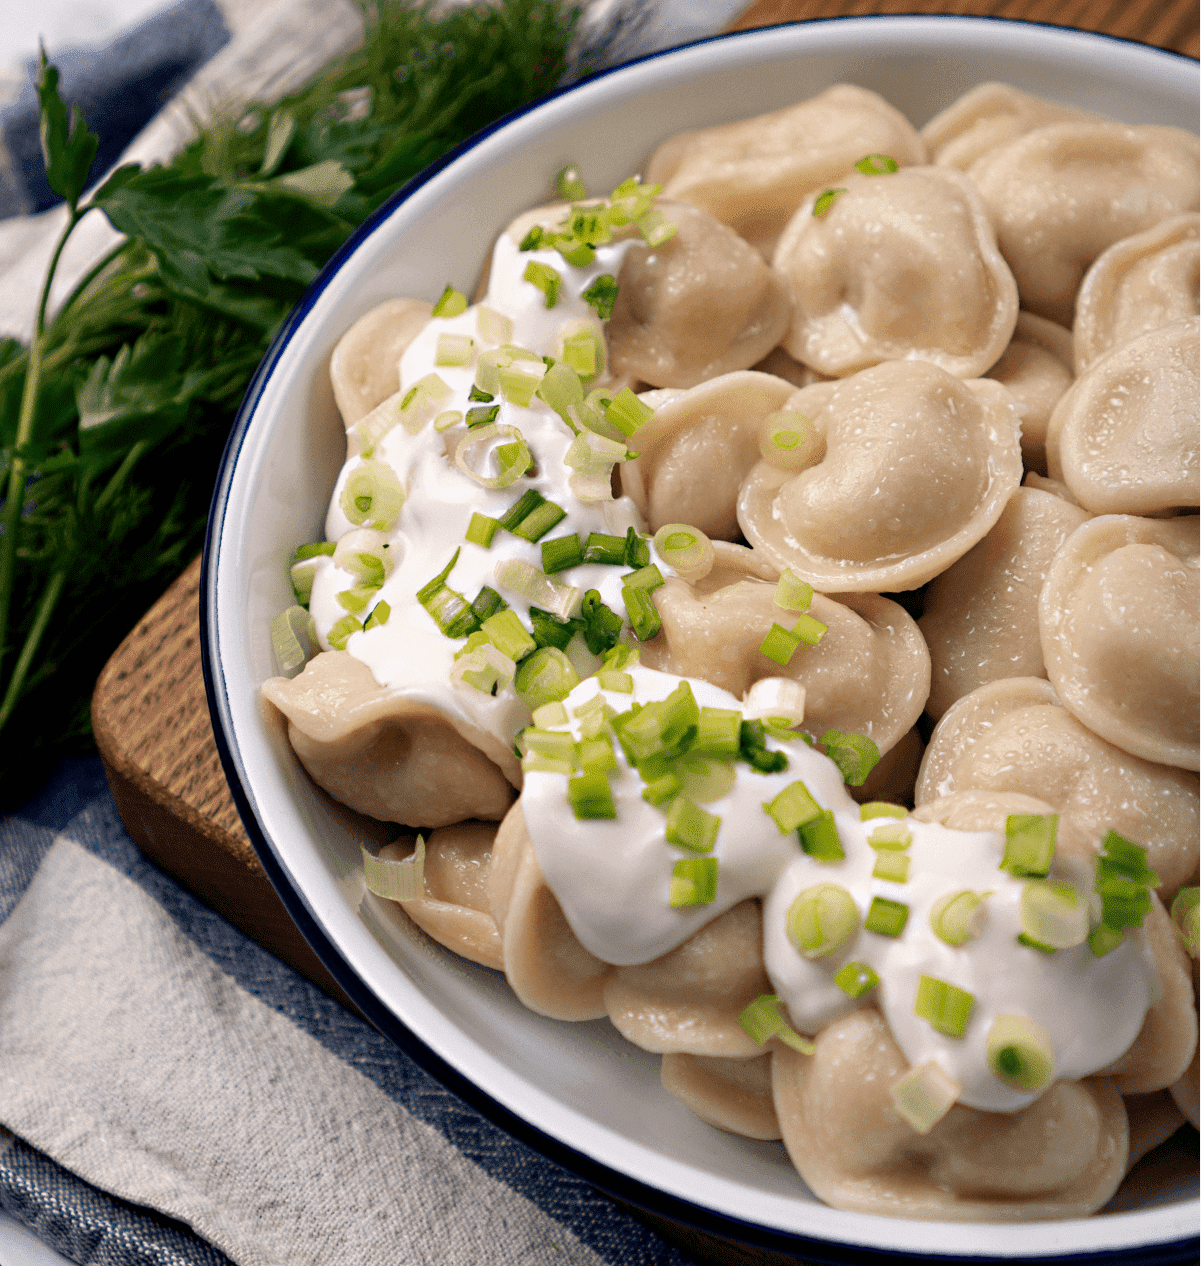
\includegraphics[width=1in]{assets/test4.png}}} \\ \hline
			
			5& jpeg & {\specialcell{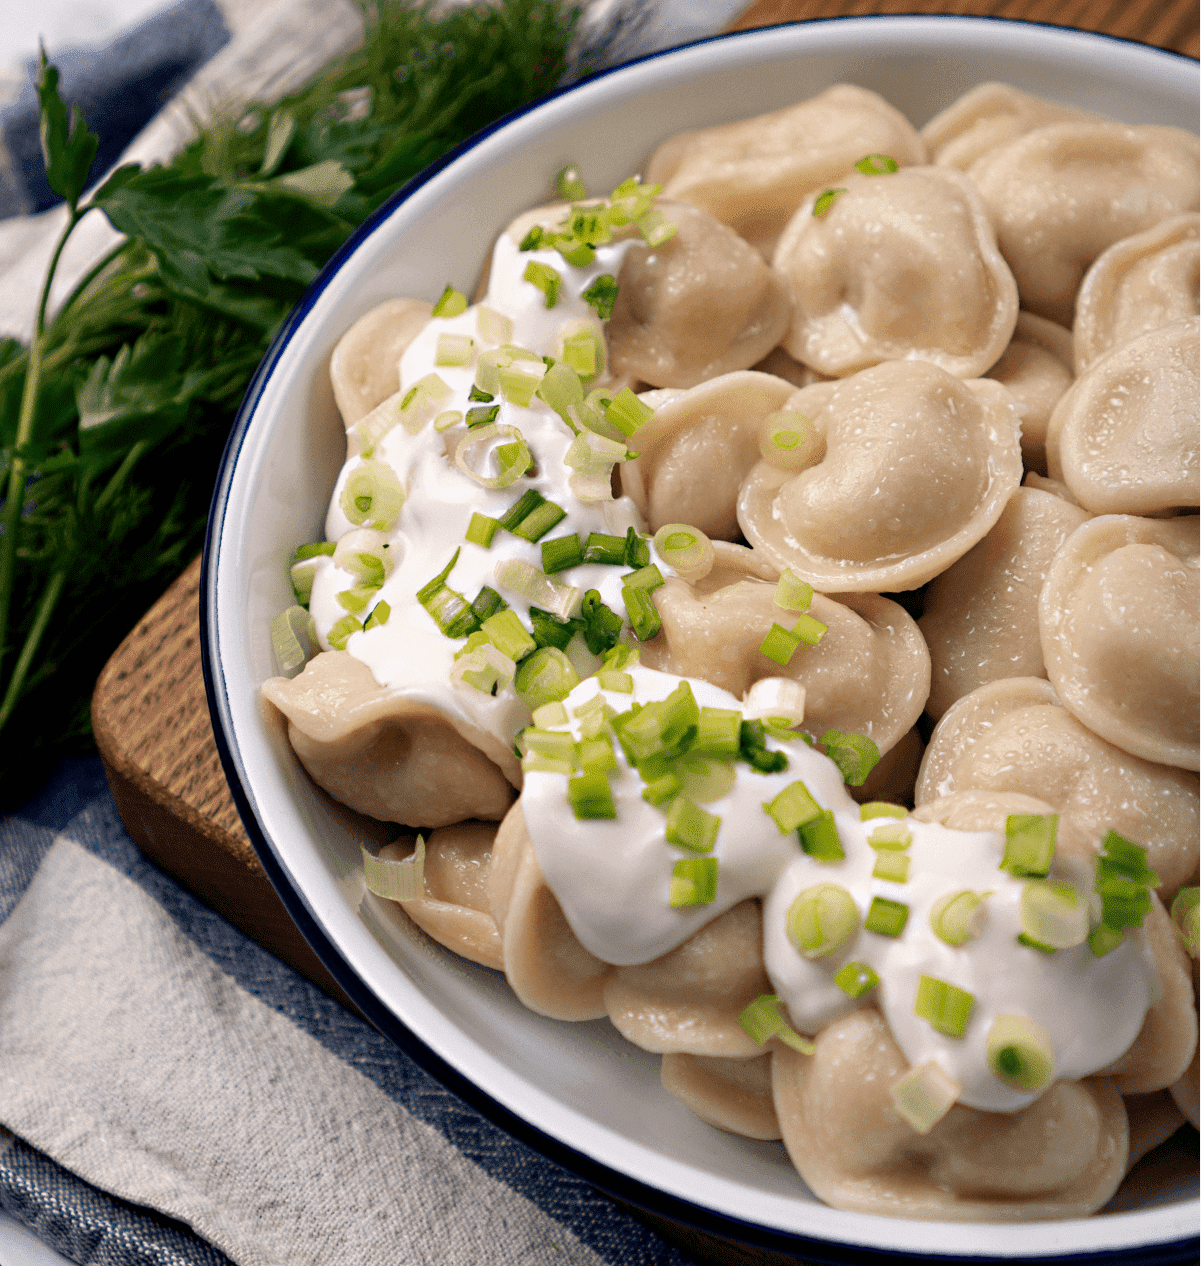
\includegraphics[width=1in]{assets/test4.png}}} \\ \hline
		
			
		\end{tabular}
	\end{center}
\end{table}

\newpage

\chapter*{Заключение}

В результате выполнения данной лабораторной работы был реализован в виде программы на языке Си алгоритм шифрования RSA и механизм цифровой подписи на основе алгоритма хеширования MD5.